\subsection{Modelling Challenges}

There are fundamental challenges that currently limit the effectiveness of modelling tropical phenomena.  The current generation of climate models (CMIP5) do not consistently predict the same results for particular phenomena.  These phenomena include precipitation patterns, SST patterns, Madden-Julian Oscillation and ENSO.  Whenever models disagree on a specific aspect of any of these phenomena, it makes future prediction must less certain.  Therefore, it is necessary to identify the deficiencies in modelling which cause the discrepancies in model results.  


\begin{figure*}[h!]
\begin{center}
  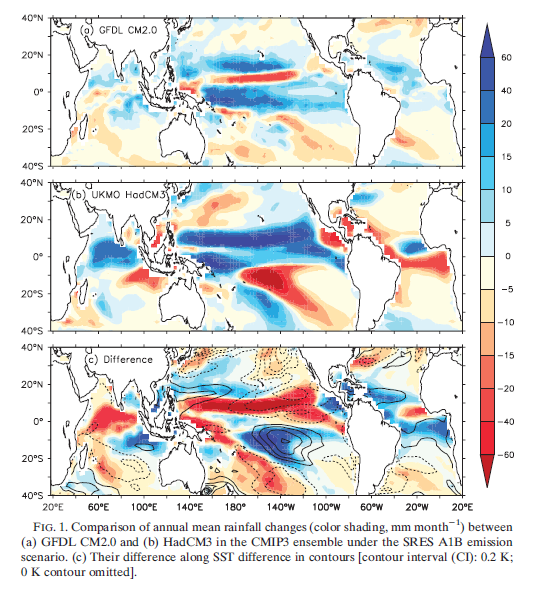
\includegraphics[width=0.790\textwidth]{isaac-fig1.png}
  \label{fig:isaac1}
\end{center}
\end{figure*}


Rainfall projections are an important aspect of tropical modelling.  According to the IPCC report, there is a wide range of inter-model variability in future rainfall projections.  Obvious model differences can be seen in Figure \ref{fig:isaac1} above.  A third of the variability was shown to be caused by differences in the SST warming pattern (Ma and Xie, 2013).  According to Ma and Xie, there is a strong correlation between warmer-than-average SST and increased precipitation within regions.  Thus modeling SST warming patterns is very important for predicting future rainfall.  While SST is projected to increase in general, the pattern of warming is not projected to be uniform.  Further, this pattern of warming is not consistent among models.  Due to the correlation of SST warming and precipitation, any inaccuracy in predicting SST warming patterns is inherited by the modelling of future rainfall.  This is a modelling challenge because SST pattern formation involves complicated processes such as ocean-atmosphere interactions and the interaction between convection and large-scale environment which are not well-understood.\\


\begin{figure*}[h!]
\begin{center}
  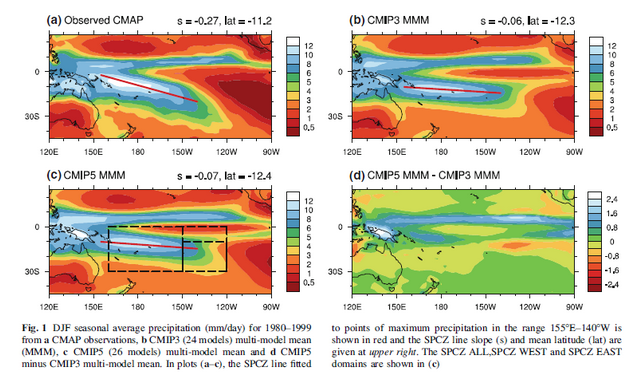
\includegraphics[width=0.790\textwidth]{isaac-fig2.png}
  \label{fig:isaac2}
\end{center}
\end{figure*}


The study of the the Intertropical Convergence Zone (ITCZ) is another modeling pursuit that is very relevant to the projection of future precipitation in the tropics.  A major issue in modelling this feature is the appearance of an unrealistic ‘double ITCZ’ pattern in many models.  \\
An example of this ‘double ITCZ’ is seen in the eastern Pacific ocean, where models project a higher level of precipitation both North and South of the equator, as opposed to reality, where a diagonally oriented convergence zone is present in the south.  This can be seen in Figure \ref{fig:isaac2} above. In a study, Brown used a regime sorting technique, in which precipitation change is decomposed into dynamic, thermodynamic, and covariant components (Brown et al., 2012).  This study showed that, in the regions where models most often disagree with reality, the dynamic and thermodynamic components of the precipitation change were also most different from reality.  This suggested that reduced atmospheric moisture and reduced ascent are to explain for the apparent bias.  In a previous study by Brown, it was shown that models that use flux adjustments are the most accurate in reproducing the observed spatial ITCZ pattern, while models that do not use flux adjustments fail to capture the diagonal orientation (Brown et al., 2011).\\

This result suggest the absence of ocean-heat flux adjustments in most CMIP5 models may be responsible for their inaccuracy in modeling the observed ITCZ pattern.  Once again, the influence of SST warming, and in this case zonal SST gradient, is an important factor in modeling another climate phenomena.\\

Considering the above result, one might wonder why more models do not use ocean-atmosphere flux adjustments, since doing so enables better modelling of the ITCZ.  The answer is there is a tradeoff.  The inclusion of ocean-atmosphere flux adjustments can cause climate drift over long periods of time within a model (Gordon et al., 2000).  If the ocean heat transports implied by atmospheric surface fluxes are significantly different from the ocean model, SST might drift to establish a new balance.  Thus, while flux adjustments might be useful for predicting ITCZ pattern, their universal effect could cause other undesirable issues.\\

Madden Julian oscillation is the dominant mode of tropical intraseasonal variability.  However, the IPCC reports that modelling of this phenomena remains challenging, leading to future projections of MJO having low confidence.  Like with precipitation change and ITCZ pattern, MJO has been shown to be highly sensitive to the pattern of SST warming (Maloney and Xie, 2012).  So, like before, the uncertainty in projecting future SST warming patterns is a leading cause of uncertainty in projecting MJO properties.\\

According to the IPCC report, most CMIP3 and CMIP5 models disagree on the response of the zonal SST gradient to the El Nino Southern Oscillation (ENSO) across the equatorial Pacific.  ENSO properties have been shown to be influenced by the background state of the tropical Pacific, which includes SST properties and the sensitivity of the atmosphere to SST changes (Yeh et al., 2012).  The magnitude of the SST trend in the tropical Pacific has been reduced from CMIP3 to CMIP5.  Yeh suggests that this change may be due to overestimation of the response to natural forcing and aerosols by including Earth system models.  If this is true, it emphasizes the need to examine how the addition of Earth System models, and their detailed physical processes, affects the larger models of which they are a part.\\

\subsection{Trends}

Within all these issues are a few common trends.  One trend is that many phenomena depend on the modelling of other phenomena.  And thus, if the modelling of one phenomena is flawed, than it would be unrealistic to expect accurate results from any phenomena that depend on it.  This is exemplified by the dependence of most tropical phenomena on the SST spatial and gradient patterns.  Since there are many questions raised about the accuracy of SST modelling, and the proper way to model (whether to use flux adjustments or not), this uncertainty extends to the modelling of precipitation patterns, ITCZ patterns, MJO, and ENSO.  While SST itself may not be very relevant to humans, the phenomena that depend on it certainly are.  Therefore, better modelling of SST is needed. \\

Another trend is the ‘trade-off’ between different modelling approaches.  Sometimes a particular approach is better at modeling a specific phenomenon than another approach.
However, this approach might have side-effects that negatively affect the model as a whole.
This is best exemplified by the tradeoff between using flux-adjustments or not.
As described above, using flux adjustments within a model can produce better results for simulating ITCZ, but as a consequence, can cause climate drift across the entire model as a whole.\\

The last trend is the importance of properly weighing the influence of various modelled processes.
If a particular process is excessively simulated its effects might exceed those seen in reality or diminish the effects of other important processes.  This is best exemplified by the overestimating of forcing that Yeh suggests is causing disparity in the SST trend of ENSO.
A key challenge in modelling is making sure some processes are not overly accounted for by multiple models.\\

Overall, the challenge for Applied Mathematicians moving forward is to better model SST in the tropics, or more specifically, better model the interaction between SST and atmosphere.  If the most advanced climate models had a more robust prediction of future SST warming, this by itself, would provide more consistency to predictions of precipitation, MJO, and ENSO.  It’s possible SST is not the only issue plaguing tropical climate predictions, but resolution of the issue would highlight the other issues which are not as noticeable at this time.\\

\subsection{References}

Brown, J., A. Moise, and R. Colman, 2012a: The South Pacific Convergence Zone in CMIP5 simulations of historical and future climate. Climate Dynamics, doi:10.1007/s00382-012-1591-x, 1-19. 

Brown JR, Power SB, Delage FP, Colman RA, Moise AF, Murphy BF
(2011) Evaluation of the South Pacific Convergence Zone in
IPCC AR4 climate model simulations of the 20th century. J Clim
24:1565–1582

Gordon, C., Cooper, C., Senior, C., Banks, H., Gregory, J., Johns,
T., Mitchell, J., and Wood, R.: The simulation of SST, sea ice extents
and ocean heat transports in a version of the Hadley Centre
coupled model without flux adjustments, Climate Dynam., 16,
147–168, 2000.

Ma, J., and S.-P. Xie, 2013: Regional patterns of sea surface temperature change: A source of uncertainty in future projections of precipitation and atmospheric circulation. Journal of Climate, 26, 2482-2501. 

Maloney, E. D., and S.-P. Xie, 2013: Sensitivity of MJO activity to the pattern of climate warming. Journal of Advances in Modeling Earth Systems, 5, 32-47. 

Yeh, S.-W., Y.-G. Ham, and J.-Y. Lee, 2012: Changes in the tropical Pacific SST Trend from CMIP3 to CMIP5 and its implication of ENSO. Journal of Climate, 25, 7764-7771. 
